
\documentclass[runningheads]{llncs}
\usepackage{graphicx}
\usepackage{apacite}
\usepackage{float}
\usepackage{listings}
\lstset{
  basicstyle=\ttfamily,
  columns=fullflexible,
  frame=single,
  breaklines=true,
  postbreak=\mbox{\textcolor{red}{$\hookrightarrow$}\space},
}
\usepackage{float}
\usepackage[table]{xcolor}
\usepackage[toc,page]{appendix}
\usepackage{ucs}
\usepackage[utf8x]{inputenc}

\usepackage{hyperref}
\hypersetup{
	colorlinks=true,
	linkcolor=blue,
	filecolor=magenta,      
	urlcolor=cyan,
}

\usepackage[slovene]{babel}
\selectlanguage{slovene}

\lstset{
    breaklines=true,
    breakatwhitespace=true,
    inputencoding=utf8,
    extendedchars=false,
}

\renewcommand{\baselinestretch}{1.2} % za boljšo berljivost večji razmak
\renewcommand{\appendixpagename}{\normalfont\Large\bfseries{Appendix}}

\begin{document}

\title{Seminarska naloga}
\subtitle{Implementacija algoritma za grupiranje in določanja vodja grupe}

\author{Danijel Maraž, Nejc Rebernik}

\institute{Fakulteta za Računalništvo in Informatiko UL
\email{dm9929@student.uni-lj.si}\\
}

\maketitle             

\begin{abstract}
The article covers the work done in the scope of the seminar assignment as part of the subject wireless sensor networks.

\keywords{Raft nRF24LO1 Leader Consensus Wemos ESP}
\end{abstract}

\section{Uvod}
Cilj projekta je bila implementacija algoritma za določanje vodje gruče brezžičnih naprav. Razvoj in testiranje sva opravljala na ploščici z WEMOS D1 mini kontrolerjem in modulom za komuniciranje nRF24L01. Na ploščici so bili nameščeni še drugi moduli, ki pa jih v obsegu najinega razvoja nisva uporabila. Modul nRF24L01 sprejema in oddaja na frekvenci 2.4GHz z maksimalno hitrostjo prenosa do 2Mbps. Majhne velikosti sporočil uporabljenih v komunikaciji in glede na to relativno velika podatkovna pretočnost sta omogočala hiter razvoj in testiranje ter skalabilnost. Za določanje vodje v gruči sva implementirala protokol RAFT. Programska koda je napisana v jeziku C++ s knjižnico za upravljanje s komunikacijskim modulom nRF24L01.

\section{Splošna struktura}
Odločila sva se, da ne bova imela več kot ene verzije kode in da se bo vsaka naprava lahko priključila na najino omrežje. Posledično je koda že sama po sebi zelo univerzalna, saj vsebuje vse kar napravi omogoča, da opravlja vse vloge RAFT protokola. Osnoven tok dogodkov sestoji iz aktivacije naprave in pogona \textit{LR\_task} in \textit{election\_task} opravil. \textit{LR\_task} opravilo je namenjeno poslušanju aktivnosti na omrežju, ter hkrati pošiljanju sporočil, ko je to potrebno. \textit{Election\_task} je za razliko samo časovnik, ki napravi sporoči, kdaj naj privzeto pošlje sporočilo. Za tako zasnovo sva se odločila, ker je posledica tega večja predvidljivost in determinizem samega programa, saj lahko samo eno opravilo pošilja oziroma sprejema.

\section{Pošiljanje in poslušanje}
Knjižnica za upravljanje z nRF24LO1 modulom predvideva za prenos podatkov uporabo programskih abstrakcij z imenom cevi (eng. pipe), ki pa so najin projekt v veliki meri ovirale, saj je imeti hkrati odprto cev za poslušanje in branje nemogoče in pa so sploh cevi namenjene neenakopravni komunikaciji torej bolj v statični situaciji master-slave. Posledično se ob vsakem klicu posebne funkcije \textit{sendMsg}, ki je namenjena pošiljanju sporočil radio modul ponovno aktivira in odpre nova pisalna cev. Enako se zgodi ob vsaki novi vrnitvi v zanko poslušanja le, da se tokrat na novo odpre poslušalna cev. Cevi imajo prav tako tudi naslove, ki pa jih nisva potrebovala in sva ves čas pisala in poslušala na nekem poljubnem privzetem naslovu. Vredno je omeniti, da sva tako komunikacijo lahko dosegla z nastavitvijo delovanja modula, ki ne predvideva uporabe avtomatskih potrditvenih paketov ob prejetju paketka, zato je scenarij v katerem se poslan paketek izgubi mogoč vendar na razdalji nekaj deset centimetrov bistveno manj verjeten.

\subsection{Election task}
Opravilo ima zelo preprosto zasnovo. Njegova glavna naloga je, da nastavi spremenljivko \textit{hastoSend} na \textit{true} in posledično sproži pošiljanje novega sporočila (nove volitve) v glavnem opravilu. Poleg tega s funkcijo \textit{changeRole} nastavi vlogo naprave na to \textit{kandidata}. 

\subsection{Listen and react task}
Ob vstopu v glavno opravilo naprava vsem ostalim članom sporoči, da se je aktivirala, ter takoj za tem začne poslušalno pisalno zanko. Naprava nato:

\begin{itemize}
\item Pod pogojem, da je \textit{kandidat} preveri, če je dobila več kot polovico glasov. V tem primeru postane novi vodja.
\item Začne poslušati in ob primeru, da obstajajo nova sporočila jih prebere ter določi kako se mora odzvati.
\end{itemize}
V najslabšem primeru bo naprava zaznala promet, ki pa ji ni namenjen (namembnost se preveri s funkcijo \textit{relevantData}) in si bo s klicem funkcij \textit{seenDevice} in \textit{removeInactiveDevs} posodobila interno tabelo naprav. \\


\subsection{Tabela naprav}
Tabela naprav je namenjena shranjevanju seznama naprav in stanja naprav v omrežju. Vsaka naprava, ki se omrežju predstavi s poslanim sporočilom se zapiše v lokalno tabelo naprav. Napravo se iz tabele odstrani, ko je njena zadnja aktivnost bila zaznana pred več kot petimi mandati. Velikost tabele sva iz praktičnih razlogov omejila na samo deset različnih naprav, vendar bi v praksi glede na najin način naslavljanja lahko ta imela do $2^{8} - 1$ naslovov.

\section{Protokol komunikacij}
\begin{figure}
  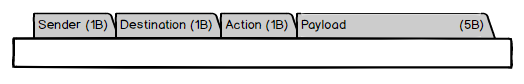
\includegraphics[width=\linewidth]{packet.png}
  \caption{Osnovna oblika paketa.}
  \label{fig:paket}
\end{figure}
Pošiljanje podatkov na radijskem modulu je omejeno na samo 8 bajtov na paket, zato sva pri implementaciji najinega dodatka aplikacijski plasti poskušala čim več bajtov nameniti koristnim informacijam, saj bi to bilo v realni situaciji zaželeno. Prvi trije bajti so namenjeni naslavljanju paketkov ter funkcij Raft protokola in sicer: \\
\begin{itemize}
\item Prvi bajt je namenjen naslovu pošiljatelja paketka. Ta je pridobljen iz zadnjega ASCII znaka MAC naslova naprave.
\item Drugi bajt je namenjen naslovu prejemnika paketka ("F" je broadcast).
\item Zadnji bajt identificira RAFT dejanje paketka.
\end{itemize}

Opis možne Raft vsebine: 
\begin{itemize}
\item A (ang. acknowledge) paket služi za potrditev prejema poljubnega sporočila, ter kot tip predstavitvenega paketa.
\item E (ang. election) paket poziva ostale naprave k glasovanju za novonastalega kandidata, ki je pošiljatelj paketa.
\item V (ang. vote) paket predstavlja glas privrženca, ki ga ta isti pošlje kandidatu in je odziv na E paket.
\item H (ang. heartbeat) paket ponastavi časovnik za nove volitve in ga pošlje vodja privržencem. V realnem svetu služi tudi za deljenje informacij med člani skupine (ang. log propagation).
\end{itemize} 


\begin{figure}
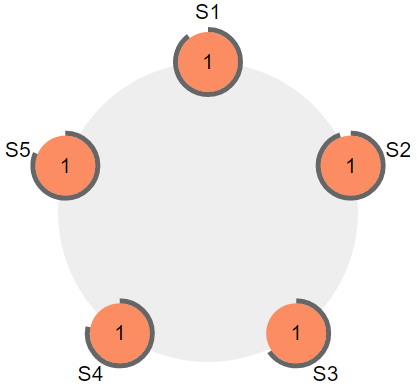
\includegraphics[scale=0.30]{raft_pics/raft1.png}
\end{figure}
\begin{figure}
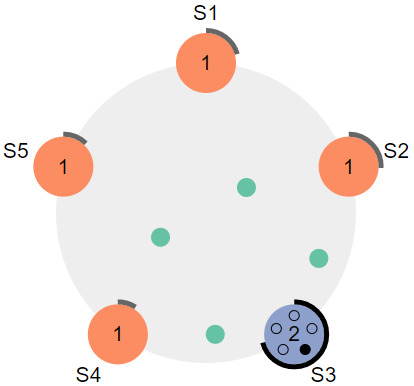
\includegraphics[scale=0.30]{raft_pics/raft2.png}
\end{figure}
\begin{figure}
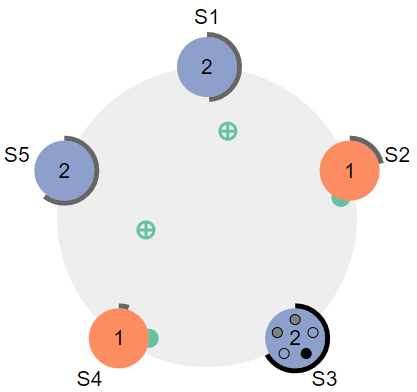
\includegraphics[scale=0.30]{raft_pics/raft3.png}
\end{figure}
\begin{figure}
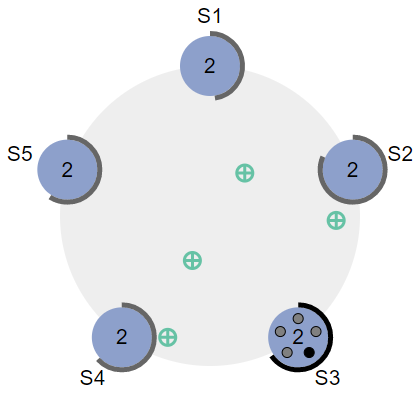
\includegraphics[scale=0.30]{raft_pics/raft4.png}
\end{figure}
\begin{figure}
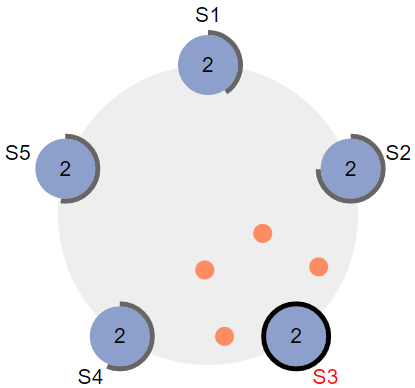
\includegraphics[scale=0.30]{raft_pics/raft5.png}
\caption{Shema tipičnega volitvenega cikla.}
\end{figure}

\section{Raft protokol}
Raft (Reliable ,Replicated ,Redundant, And Fault-Tolerant) je algoritem za sklepanje soglasja v porazdeljenih sistemih z več vozlišči. Narejen je bil leta 2014 z mislijo, da bo v veliki meri nadomestil starejši in veliko bolj zapleten Paxos algoritem. Omenjeno soglasje Raft doseže s pomočjo izvolitev vodilnega vozlišča. Naprava ima lahko v Raft skupini eno izmed treh vlog: \\
\begin{itemize}
\item Vodja (ang. leader)
\item Privrženec (ang. follower)
\item Kandidat (ang. candidate)
\end{itemize}
Odgovornost vodje je, da privržencem redno pošilja sporočila, da je ta še vedno aktiven (ang. heartbeat). Med tem ima vsak privrženec poljubni časovni interval (navadno med 150 ms - 300 ms), ki mu ob izteku spremeni vlogo v tisto kandidata ter sproži nove volitve. Če privrženec prejme potrditev, da je vodja aktiven pred iztekom časovnega intervala se časovni interval ponastavi. Pri Raftu je važna tudi kvaliteta posameznega vodje, zato se čas beleži v mandatih. En mandat je (enako kot v svetu politike) trajanje aktivnosti enega vodje oziroma potek enih volitev. V idealni situaciji bomo torej imeli samo en mandat, ker se naš vodja ne bo nikoli pokvaril. V praksi temu ni tako in številka mandata se poveča ob začetku vsakih novih volitev. 
\subsection{Volitve} 
Za izvolitev mora kandidat pridobiti več kot polovico glasov. Ko naprava postane kandidat voli zase ter sporoči ostalim, da je prišel čas za nove volitve. Privrženci se na ta klic odzovejo ter oddajo svoj glas. Včasih izvolitev kandidata ne uspe bodisi, ker je prišlo do aktivacije dveh kandidatov (v takem primeru postaneta ponovno privrženca) in posledično delitve glasov ali, ker je imel kandidat manjši števec mandata kot večina privržencev. Privrženci lahko glasujejo samo enkrat na mandat in to naredijo pod pogojem, da je številka mandata kandidata večja ali enaka njihovemu lokalnemu števcu. Vredno je omeniti, da se scenariju dveh sočasnih kandidatov da izogniti z uporabo naključnih števcev za štetje časa pred ponovnim kandidiranjem. Tako je verjetnost, da bo prišlo do dveh sočasnih volitvenih kampanj bistveno manjša.

\subsection{Naša implementacija}
Naša implementacija sledi strukturi Raft protokola z nekaj izjemami: \\
\begin{itemize}
\item Odločila sva se opustiti kvalitativne izbire vodje na podlagi številke mandata, saj pri merjenju le 5 bajtov informacij to ni zelo pomembno in bi vodja v realnem svetu gotovo pošiljal podatke kam drugam. Vodja tudi ne beleži bistveno več informacij kot privrženec.
\item Štetje mandatov je prilagojeno in kot mandat štejemo tudi uspešno poslano sporočilo, da je vodja še aktiven, ki resetira časovnike naprav.
\item Naprave ob prejetju sporočila, da je vodja še aktiven vsem napravam pošljejo potrditveno sporočilo. Tako lahko vsaka naprava vodi evidenco aktivnih naprav in se naprave v mirovanju, torej tiste, ki prejemajo heartbeat sporočilo ne zbrišejo iz tabele naprav.
\item Trajanje volitvenih ciklov je prilagojeno in sicer se privržencev časovnik giba med 2 do 5 sekundami. Za razliko ima vodja frekvenco pošiljanja potrditvenega paketa 1 sekundo. Za to sva se odločila, ker je tako bistveno lepše razvidno kaj se trenutno dogaja v omrežju.
\end{itemize}


\section{One time pad}
Sistemu sva dodala nivo varnosti s kriptiranjem sporočil z metodo one-time pad. Metodo sva izbrala zaradi  enostavnosti in majhne računske zahtevnosti, kar je pomemben faktor pri procesorjih z nizko močjo in omejitvami napajanja. One-time pad je kriptografska metoda, ki nad biti sporočila pri šifriranju in dešifriranju izvede XOR operacijo s ključem iste dolžine. V implementaciji sva uporabila statičen ključ dolžine 8 bajtov. Za tak pristop sva se odločila zaradi nezaželene zapletenosti, ki bi jo prineslo dinamično izmenjevanje ključev. To med drugim tudi omogoča visok nivo fleksibilnosti, saj lahko naprava kadarkoli izpade ter se kasneje priklopi v omrežje brez kakšnegakoli izmenjevanja ključev. \\
Uporaba istega ključa pa bi bila v kakšnem bolj resnem in zaupnem sistemu nepredstavljiva, saj lahko napadalec z zajetjem samo dveh spročil dobi XOR vrednost njunih čistopisov. Naš sistem k večjemu zagotavlja zaupnost z nejasnostjo razumevanja sistema (ang. security by obscurity). Zagotavlja pa ne integritete, saj lahko napadalec prav tako spreminja bite kriptiranih sporočil brez, da bi to mi opazili. Prav tako sistemu manjka avtentikacija, saj lahko napadalec nezaznano pošilja zajete pakete napravam. \\
$m1 \oplus key = c1$\\
$m2 \oplus key = c2$\\
$c1 \oplus c2 = m1 \oplus key \oplus m2 \oplus key = m1 \oplus m2 $ 


\section{Zaključek}
Uspelo nama je implementirati najinim ciljem primerno verzijo Raft protokola. Pri tem sva spoznala razliko med razvijanjem aplikacij za kontrolerje ter običajne višje nivojske sisteme. Lahko rečeva, da je pri prvih delovni tok precej drugačen, saj je tudi način razhroščevanja drugačen, zaradi prisotnosti nizko nivojskih fizičnih elementov kot so radijski oddajniki in interference iz okolja. Sledi nekaj bistvenih dosežkov projekta: \\
\begin{itemize}
\item Delujoč Raft protokol 
\item Enoličnost kode med napravami (skalabilnost)
\item Možnost poljubnega priklopa naprav v omrežje (fleksibilnost)
\item Zagotovitev omejene zaupnosti z one-time pad
\end{itemize}

Projekt bi lahko tudi zlahka nadgradili in sicer z dodatkom:
\begin{itemize}
\item Izmenjevanja in generacije krptografskih ključev z Diffie-Hellman protokolom
\item Pravo Raft implementacijo, ki vključuje izbiro najboljšega možnega vodje
\item Funkcionalnostjo pošiljanja dejanskih podatkov z enim izmed senzorjev npr. temperaturo
\item Pošiljanje podatkov na zunanji spletni strežnik
\end{itemize}

\section{Primera}
Za lažjo predstavo dogodkov sva sistemu dodala užiganje LED diod glede na vlogo naprave.
\begin{itemize}
\item Vodja - 3 diode
\item Kandidat - 2 diodi
\item Privrženec - 1 dioda
\end{itemize}
\begin{figure}
  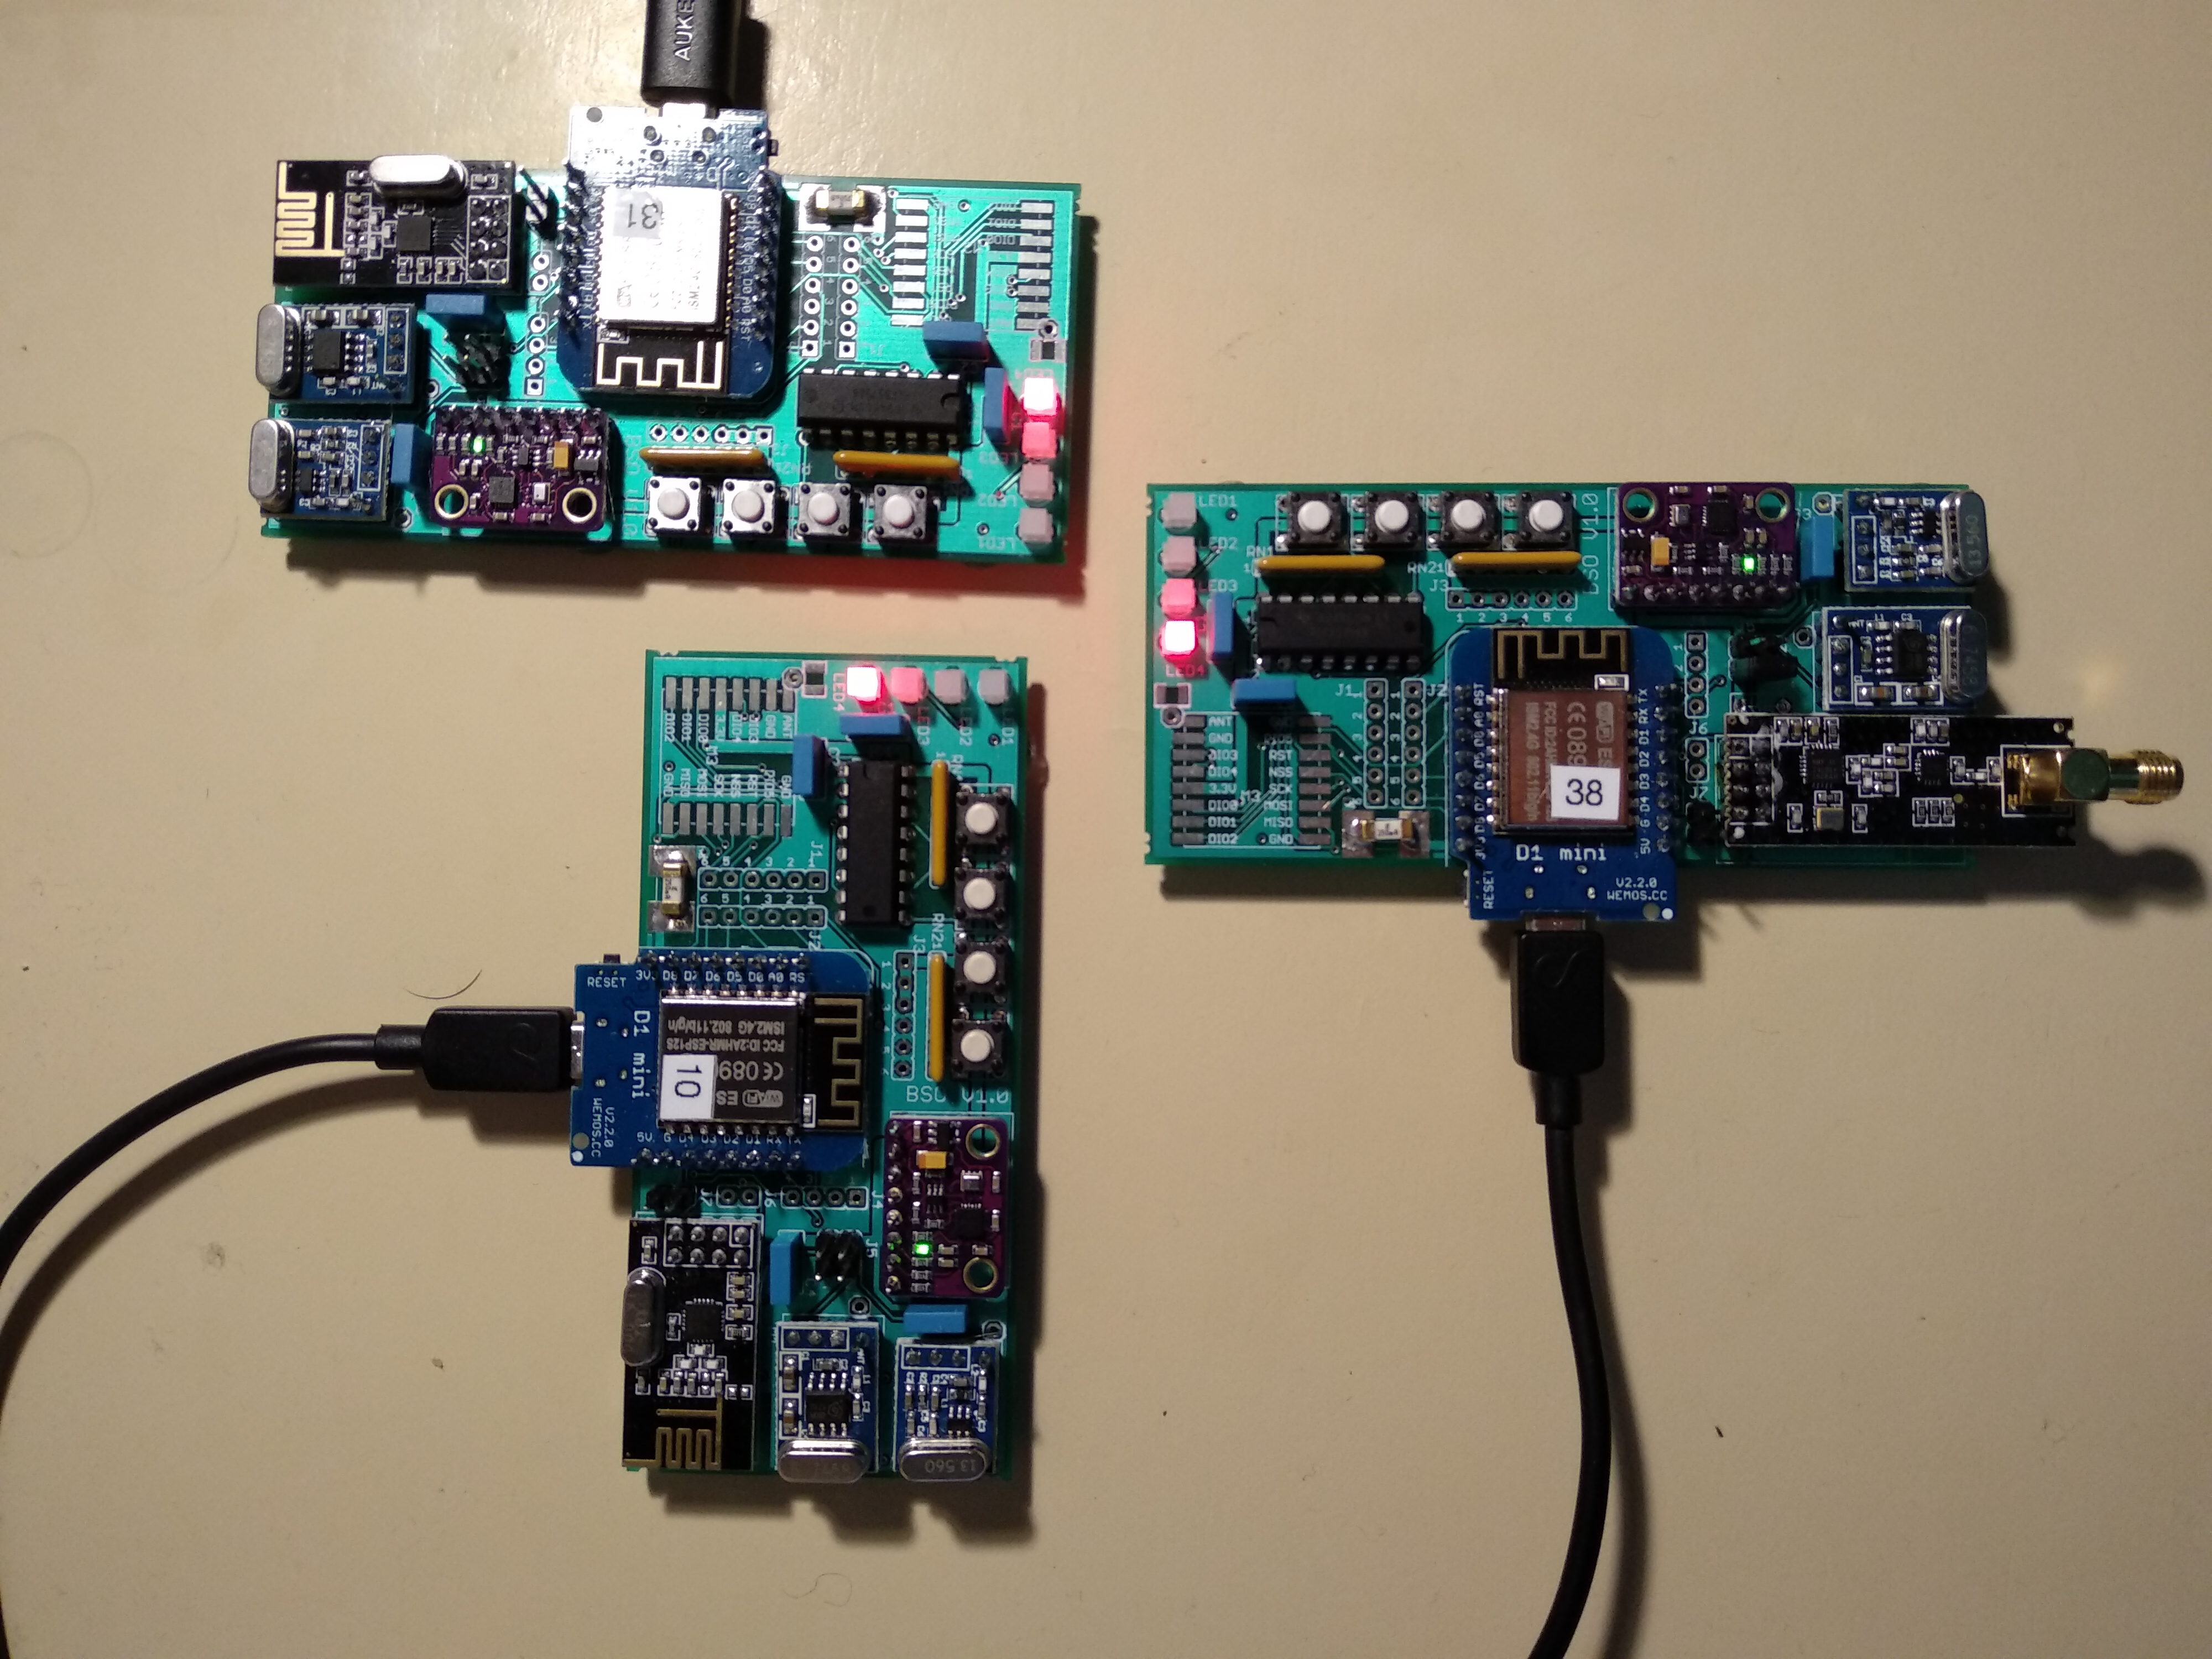
\includegraphics[width=\linewidth]{no_leader.jpg}
  \caption{Brez vodje bodo kmalu sledile nove volitve.}
  \label{fig:no_leader}
\end{figure}
\begin{figure}
  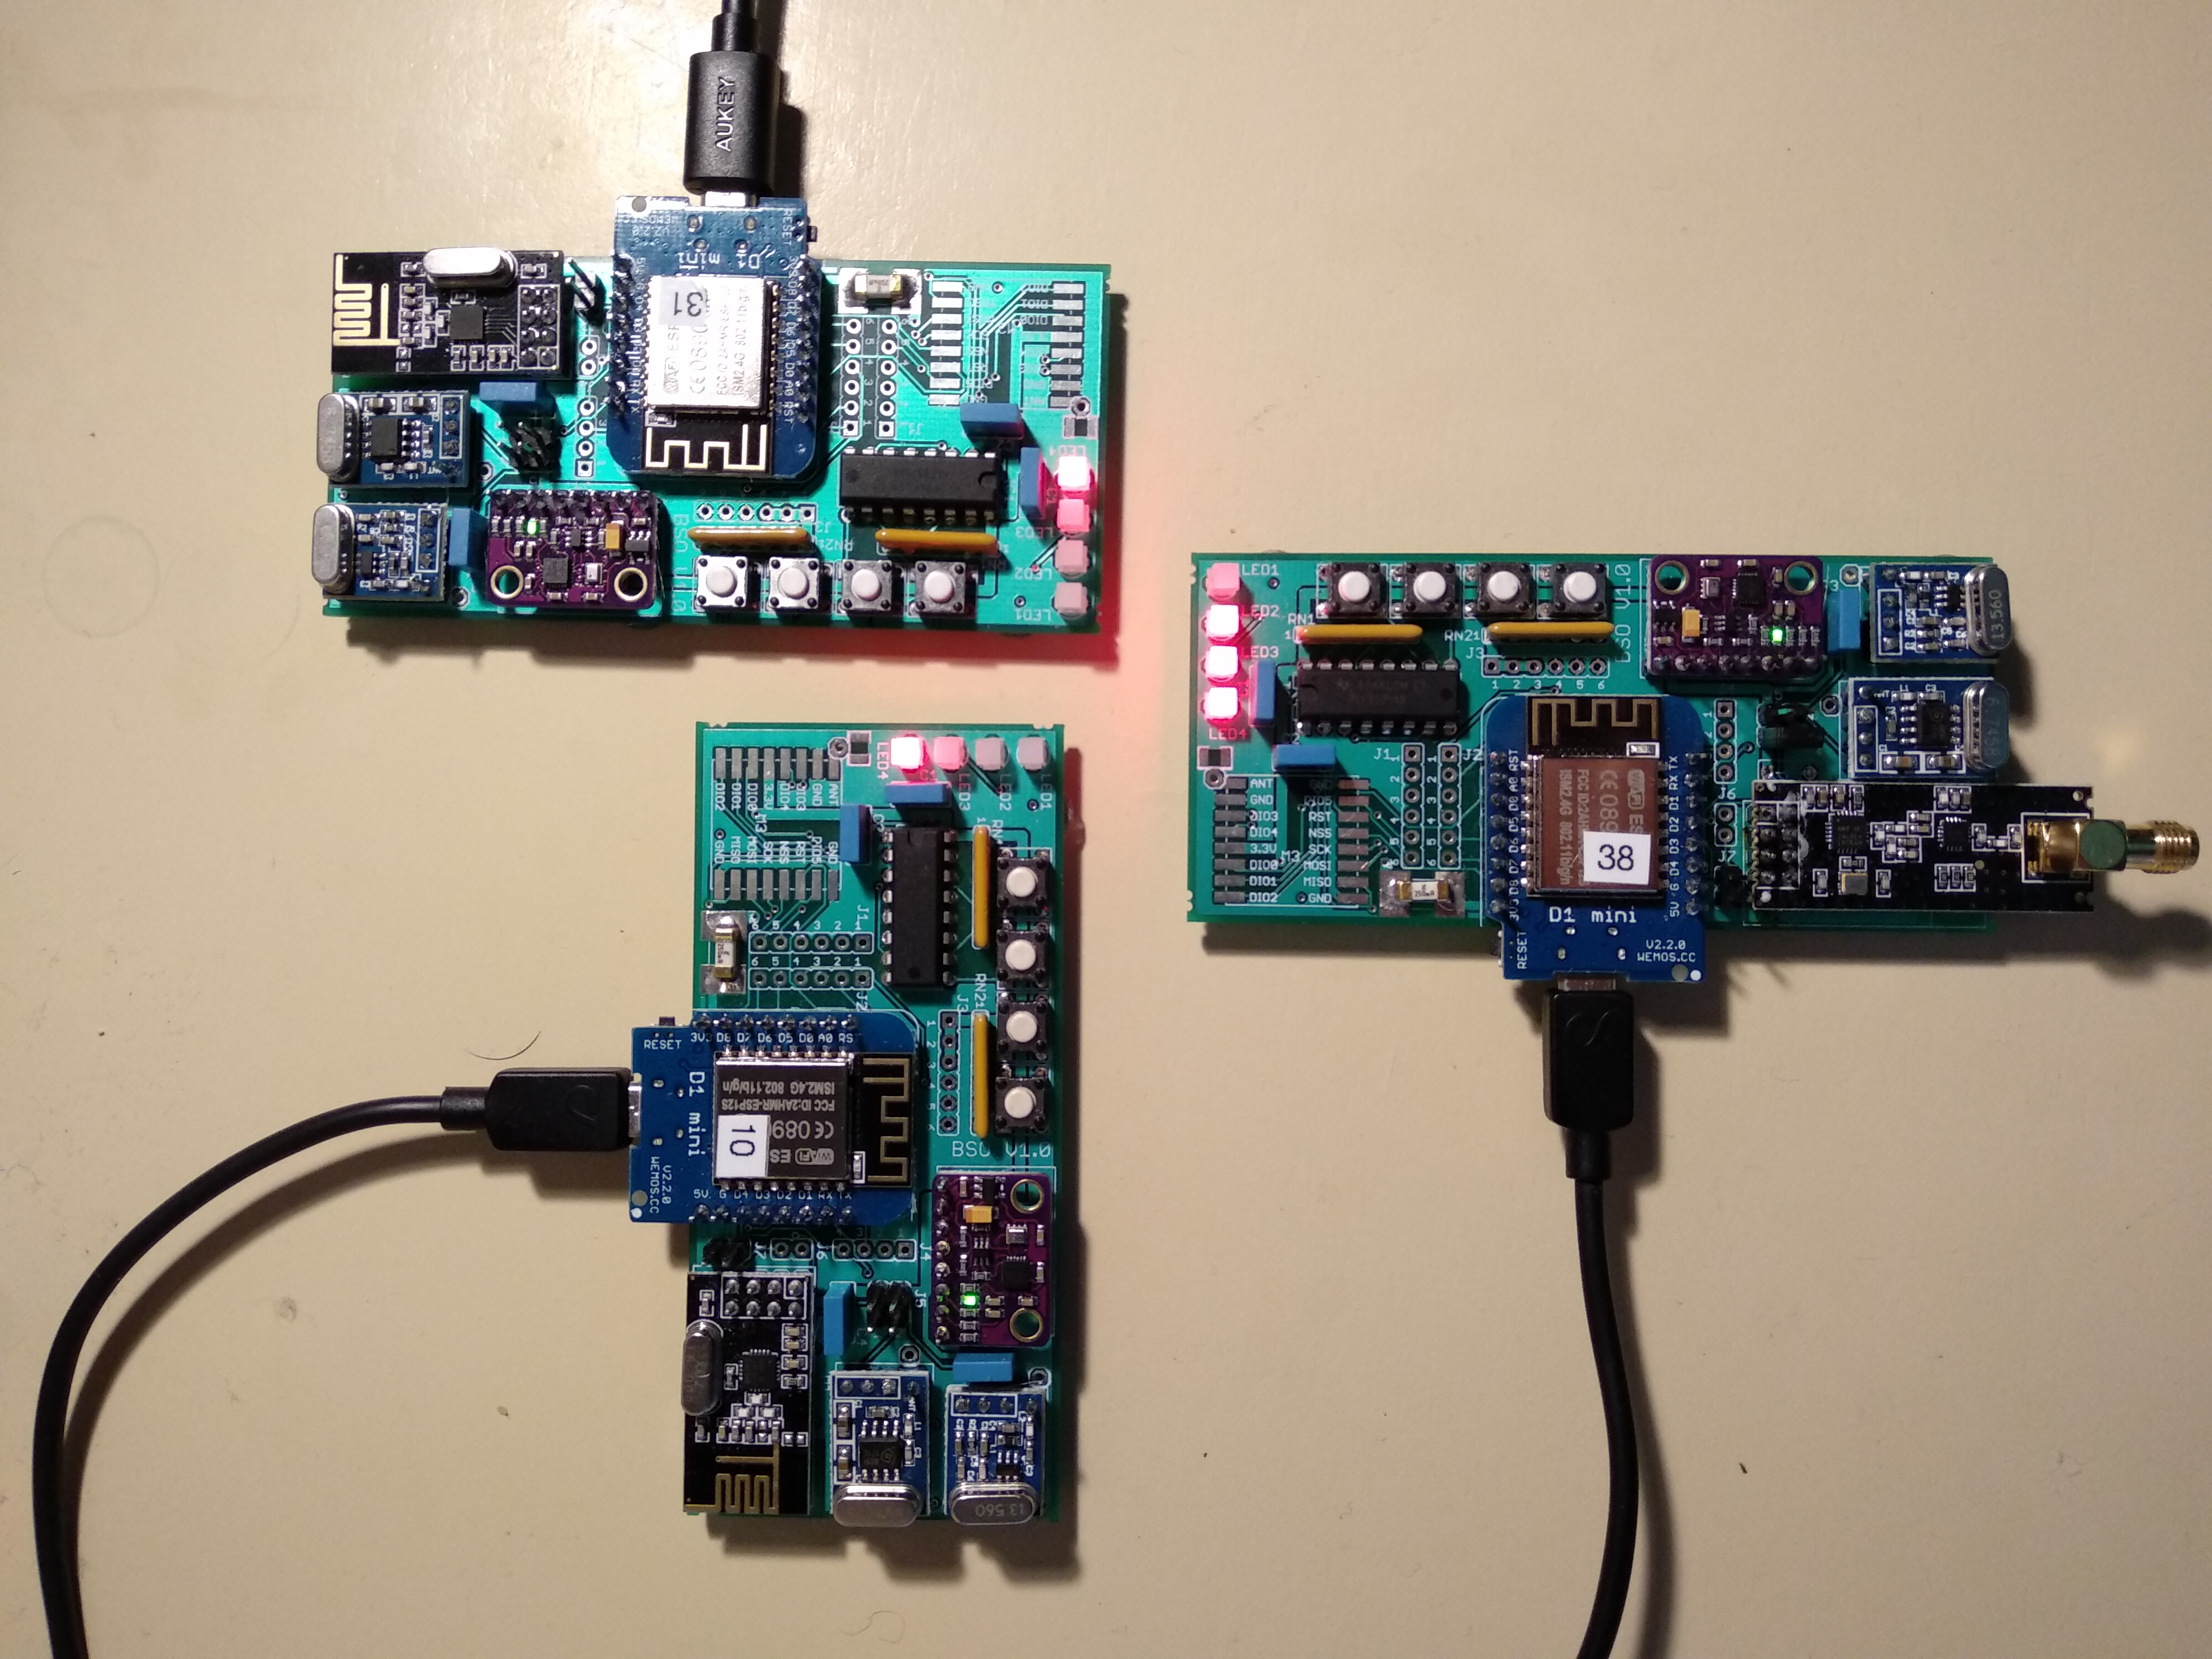
\includegraphics[width=\linewidth]{one_leader.jpg}
  \caption{Prisotnost vodje.}
  \label{fig:one_leader}
\end{figure}


\end{document}

